\documentclass[a4paper,12pt]{article}

\usepackage{amsmath, amssymb, fancyhdr, geometry, framed, graphicx}
\geometry{left=1.5cm, right=1.5cm, top=2cm, bottom=2cm}
\pagestyle{fancy}
\fancyhf{}
\rfoot{\thepage}
\renewcommand{\headrulewidth}{0pt} % Remove the top header line
\renewcommand{\footrulewidth}{0.4pt} % Add a line for footer

% Custom title box
\newsavebox{\titlebox}
\sbox{\titlebox}{
    \begin{minipage}{\textwidth}
        \begin{center}
            \fbox{
                \parbox{0.9\textwidth}{
                    \centering
                    \small
                    \textbf{COMP3008J Distributed Systems \\ Tutorial \#3}
                }
            }
        \end{center}
    \end{minipage}
}

\begin{document}

% Custom title
\center{
\vspace*{-1.5cm} % Move title closer to the top
\usebox{\titlebox}

% Date and Name Section
\vspace{0.8cm}
\noindent Date: \underline{\hspace{2cm}2022.04.26} \hspace{2cm} Name: \underline{\hspace{2cm}Beihai ZHANG}
}

\vspace{-0.1cm}

\section*{Answers}

\begin{enumerate}
    \item \textbf{Routing:} \\
    Provide your answer here.

    \item \textbf{Overlay:} \\
    Provide your answer here.

    \item \textbf{Analyze the following network diagram:} \\
    Refer to the network diagram below and provide your analysis. Include routing paths and other observations. \\
    \vspace{0.5cm}
    \begin{center}
        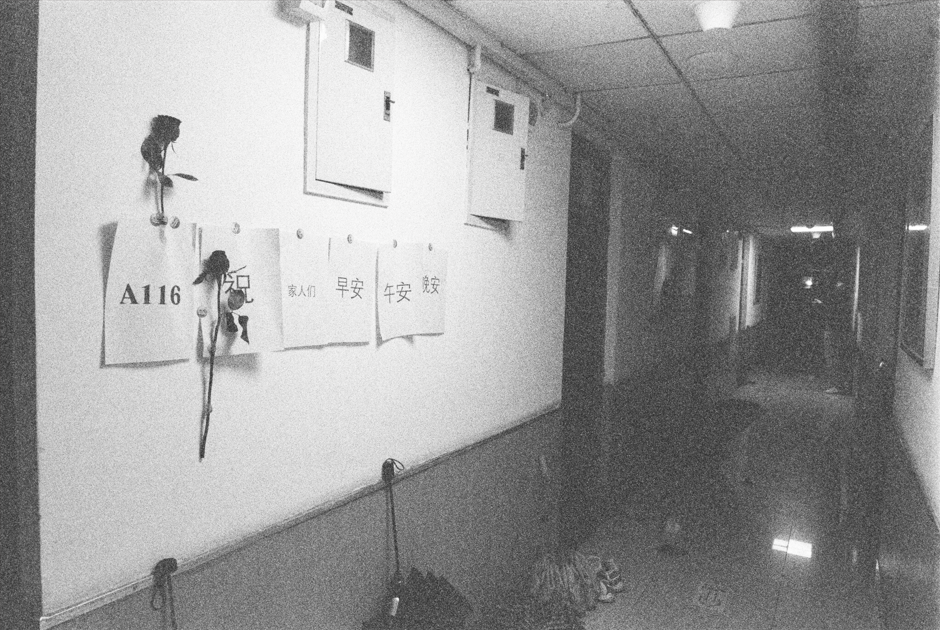
\includegraphics[width=0.8\textwidth]{images/example-network.png} % Replace with your actual image file
    \end{center}
    \vspace{0.5cm}
    [Provide your analysis here.]

    \item \textbf{Fill in the table below:} \\
    Complete the table with the appropriate values for the given scenario.

    \vspace{0.5cm}
    \begin{center}
        \begin{tabular}{|c|c|c|c|}
            \hline
            Parameter & Node A & Node B & Node C \\ \hline
            Latency (ms) & \underline{\hspace{2cm}} & \underline{\hspace{2cm}} & \underline{\hspace{2cm}} \\ \hline
            Packet Loss (\%) & \underline{\hspace{2cm}} & \underline{\hspace{2cm}} & \underline{\hspace{2cm}} \\ \hline
            Bandwidth (Mbps) & \underline{\hspace{2cm}} & \underline{\hspace{2cm}} & \underline{\hspace{2cm}} \\ \hline
        \end{tabular}
    \end{center}
    \vspace{0.5cm}
    [Provide your explanation here.]

\end{enumerate}

\end{document}



